\section{Autoencoders}
Autoencoders are a subset of neural networks. Whereas a general neural network
 in principle can take any shape, autoencoders are more restrictive.
This restrictiveness can in its most general sence we condensed 
into the following points:
\begin{itemize}
    \item Same number of output categories as input categories  
    \item A latent space with smaller dimensionality than the input/output layer  
\end{itemize}
What we end up with two funnel shaped parts linked together. The two funnels are 
called the encoder (left funnel) and decoder (right funnel) respectively. This architecture is not 
accidental, but rather designed with a very specific solution of ploblems in mind, reconstruction. 
A good example to illustrate this is image reconstruction, illustrated in figure \ref{fig:ae_denoise}. 
Suppose you have an image, and want to reconstruct it. By feeding the encoder an image, 
and comparing the decoder output to the actual image, the autoencoder can tune itself to recreate the images it trains on. 

\begin{figure}[h!]
    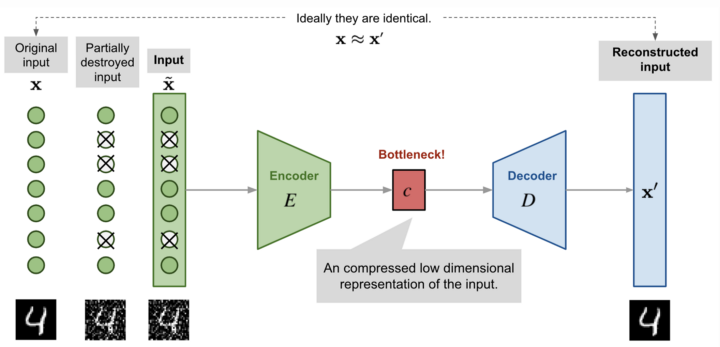
\includegraphics[width=\linewidth]{Figures/Machinelearning/autoencoder_imagedenoising.png}
    \caption{Figure depicting a model for an autoencoder. Here the input $\bf{x}$ is the original image, $\bf{x'}$ is a reconstructed version of $\bf{x}$, $g_{\phi}$ is the encoder, $f_{\theta}$ is the decoder, and $z$ is the latent space. Found 14.01.23 \href{https://lilianweng.github.io/posts/2018-08-12-vae/autoencoder-architecture.png}{here} \cite{weng2018VAE}. }
    \label{fig:ae_denoise}
\end{figure}

Mathematically this is is represented as follows\cite{weng2018VAE}. Using the annotations of each component in figure \ref{fig:ae_denoise}
we have that the decoded information is defined as follows 
\begin{equation*}
    \bf{z} = g_{\phi}(\bf{x}),
\end{equation*}    
and the reconstruction given as 

\begin{equation*}
    \bf{x'} = f_{\theta}(g_{\phi}(\bf{x})).
\end{equation*}  

The parameters $(\phi,\theta)$ are the tuneable parameters adjusted according to the loss function. In our case, the goal is
reconstruction without copying, thus we can simply use mean squared error, given as 

\begin{equation}\label{eq:loss_ae}
    L_{AE} (\phi,\theta) = \frac{1}{N}\sum_{i=0}^{N-1} \left(\bf{x}^{i} - f_{\theta}(g_{\phi}(\bf{x}^{i}))\right)^{2}.
\end{equation}

\section{Variational autoencoders}
Another popular method for reconstruction is the so called variational autoencoder. The work by Kingman and Welling \cite{VAE} showed how
one can use the variational bayesian approach for efficient approximate posterior inference, leading to the use of variational autoencoders.
\subsection*{Variational Bayes}




\subsection*{Variational autoencoders}
Now, this variational bayes can then be used to create a variational autoencoder. This contains two neural networks, the generative model $p_{\theta}(x,z)$,
as well as the probabilistic encoder $q_{\phi}(z|x)$, which is used to approximate the posterior $p_{\theta}(z|x)$. We now let the prior over 
the latent space be a multivariate Gaussian, lacking parameters: $p_{\theta}(z) = \mathcal{N}(z;0,I)$. We also have that $p_{\theta}(x|z)$ is a multivariate Gaussian,
with a distribution generated from z, whilst $p_{\theta}(z|x)$ is in fact intractable. If we now assume that the true (intractable) posterior 
is a Gaussian with approximately diagonal convariance, we can let the variational approximate posterior be a multivatiate Gaussian:
\begin{equation}
    log\, q_{\theta}(z|x^{(i)}) = log\, \mathcal{N}(z;\mu^{(i)},\sigma^{2(i)}I),
\end{equation}
where the mean and standard deviation are given by the neural network. Now, we sample from the approximate posterior $z^{(i,l)} \thicksim q_{\theta}(z|x^{(i)})$
where $z^{(i,l)} = g_{\phi}(x^{(i)}, \epsilon^{(l)}) = \mu^{(i)} + \sigma^{(i)} \odot \epsilon^{(l)}$, $\epsilon^{(l)} \thicksim \mathcal(N)(0,I)$ and $\odot$
is the elementwise product. If both the prior $p_{\theta}(z)$ and $q_{\theta}(z|x)$ are Gaussian, the KL divergence can be computed analytically, and it 
can then be showed\footnote{VURDER Å LEGGE TIL UTREGNINGEN I APPENDIX}\cite{VAE} that the variational approximate posterior is:

\begin{equation}\label{eq:loss_vae}
    \mathcal{L}(\theta, \phi;x^{(i)}) \simeq \frac{1}{2}\sum_{j=1}^{J}(1 + log\, ((\sigma^{(i)}_{j})^2) - (\mu^{(i)}_{j})^2 - (\sigma^{(i)}_{j})^2) +\frac{1}{L}\sum_{l=1}^{L}log\, p_{\theta}(x^{(i)}|z^{(i,l)}),
\end{equation}

where $z^{(i,l)} = \mu^{(i)} + \sigma^{(i)} \odot \epsilon^{(l)}$ and $ \epsilon^{(l)} \thicksim \mathcal{N}(0,I)$.

\begin{figure}[h!]
    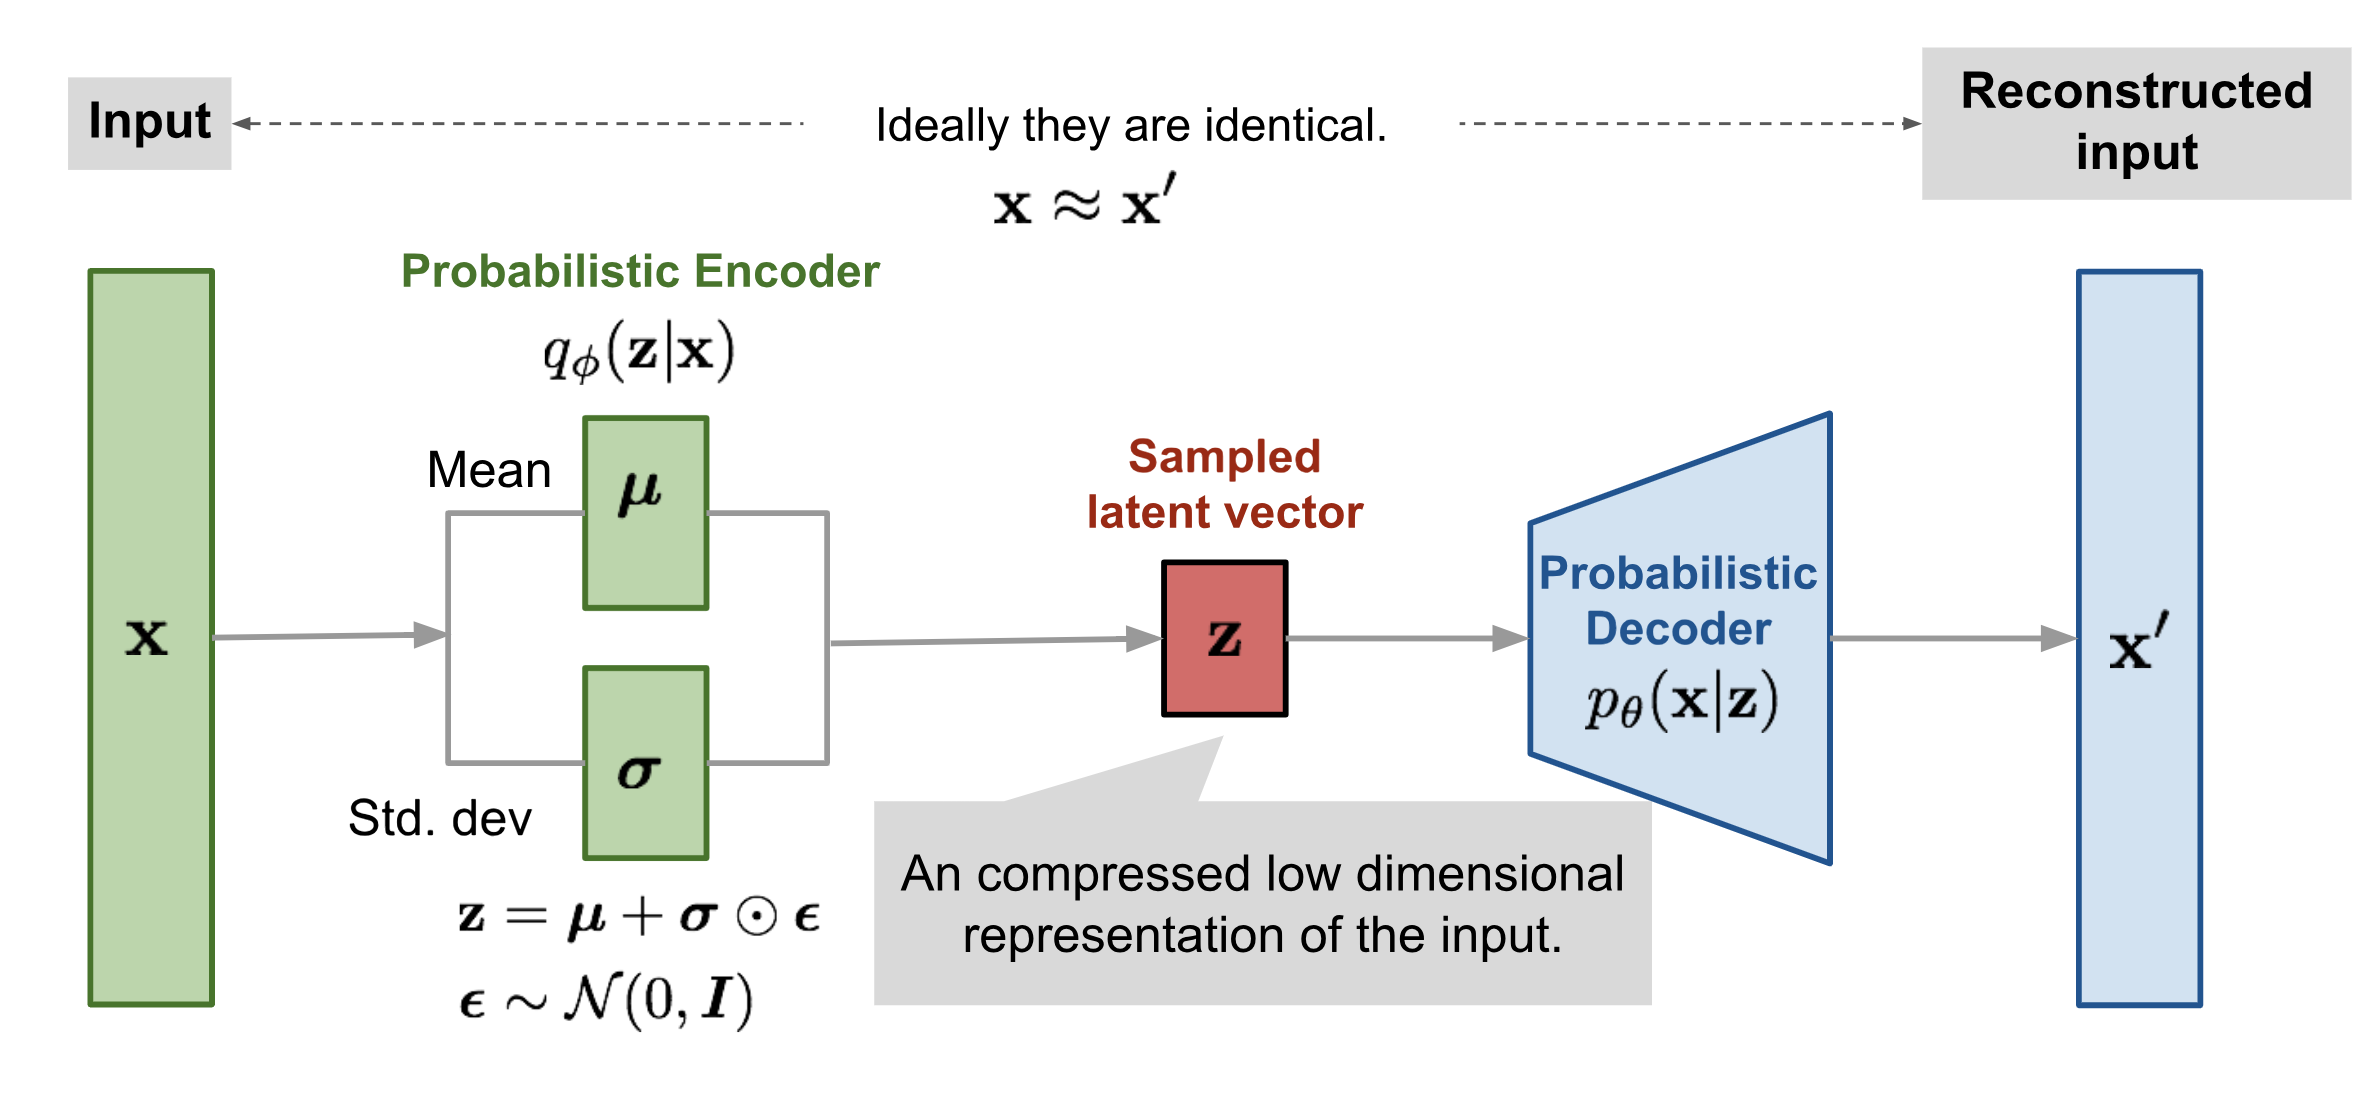
\includegraphics[width=\linewidth]{Figures/Machinelearning/vae-gaussian.png}
    \caption{Figure depicting a model for a variational autoencoder. Found 14.01.23 \href{https://lilianweng.github.io/posts/2018-08-12-vae/vae-gaussian.png}{here} \cite{weng2018VAE}. }
    \label{fig:vae}
\end{figure}

Figure \ref{fig:vae} is a graphical representation of the variational autoencoder. The encoder is a neural network, which takes 
the input $\bf{x}$ and maps the input to a latent space by creating a Gaussian distribution. The decoder is a neural network, 
which takes the latent space $\bf{z}$ and outputs the parameters of a Gaussian distribution for the data.
The loss function is given by equation \ref{eq:loss_vae}.